% vim: set textwidth=78 autoindent:

\subsection{Coordinate Capture Plugin}

% when the revision of a section has been finalized, 
% comment out the following line:
% \updatedisclaimer

The coordinate capture plugin is easy to use and provides the 
capability to display coordinates on the map canvas for two 
selected Coordinate Reference Systems (CRS). You can click a 
certain point and copy the coordinates to the clipboard or you 
use the mouse tracking functionality 

\begin{figure}[ht]
   \begin{center}
   \caption{Coordinate Cature Plugin \nixcaption}\label{fig:coordinate_capture_dialog}\smallskip
   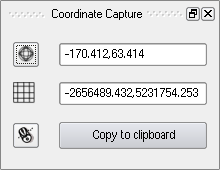
\includegraphics[clip=true]{coordinate_capture_dialog}
\end{center}  
\end{figure}

\begin{enumerate}
  \item Start QGIS, select \dropmenuopttwo{mActionOptions}{Project Properties} from 
  the \mainmenuopt{Settings} menu and click on the \tab{Projection} tab. As an alternative you 
  you can also click on the \toolbtntwo{mIconProjectionEnabled}{projector} icon in the lower 
  right-hand corner of the statusbar.
  \item Click on the \checkbox{Enable on the fly projection} checkbox and select the projected 
  coordinate system \filename{"NAD27/Alaska Albers"} with EPSG 2964 (see also 
  Section \ref{label_projections}).
  \item Load the \filename{alaska.shp} vector layer from the qgis sample dataset.
  \item Load the coordinate capture plugin in the Plugin Manager (see Section 
  \ref{sec:load_core_plugin}) and click on the \toolbtntwo{coordinate_capture}{Coordinate Capture} 
  icon. The cordinate capture dialog appears as shown in Figure \ref{fig:coordinate_capture_dialog}.
  \item Click on the \toolbtntwo{geographic}{Click to the select the CRS to use for coordinate display} 
  icon and select Geographic Coordinate System \filename{WGS84} (EPSG 4326).
  \item You can now click anywhere on the map canvas and the plugin will show the 
  \filename{"NAD27/Alaska Albers"} and \filename{WGS84} coordinates for your selected points as shown in 
  Figure \ref{fig:coordinate_capture_dialog}.
  \item To enable mouse coordinate tracking click the \toolbtntwo{tracking}{mouse tracking} icon.
  \item You can also copy selected coordinates to the clipboard.
\end{enumerate}

\newpage



